
\documentclass[5p,sort&compress]{elsarticle}

\makeatletter
\def\ps@pprintTitle{%
 \let\@oddhead\@empty
 \let\@evenhead\@empty
 \def\@oddfoot{\footnotesize\itshape
       
       \hfill\today}%
 \let\@evenfoot\@oddfoot}
\makeatother

\usepackage[utf8]{inputenc}
\usepackage[T1]{fontenc}
\usepackage{textcomp}

\usepackage{lmodern}

\usepackage[english]{babel}
\usepackage[fixlanguage]{babelbib}

\usepackage[babel=true]{microtype}

\usepackage{amsmath}
\usepackage{amssymb}
\usepackage{bm}

\usepackage{siunitx}

\sisetup{
exponent-product = \cdot,
separate-uncertainty = true,
per-mode = symbol,
group-digits = false,
}

\usepackage{graphicx}
\renewcommand{\topfraction}{.85}
\renewcommand{\bottomfraction}{.7}
\renewcommand{\textfraction}{.15}
\renewcommand{\floatpagefraction}{.66}
\setcounter{topnumber}{3}
\setcounter{bottomnumber}{2}
\setcounter{totalnumber}{10}
\usepackage{flafter}
\usepackage{booktabs}
\usepackage{multirow}
\usepackage[font=small,labelfont=bf]{caption}

\usepackage[colorlinks=true,allcolors=blue]{hyperref}

\urlstyle{same}

\begin{document}

\begin{frontmatter}

\title{TFY4240 Semester Assignment}

\author[fysikk]{V.~Hennestad}

\address[fysikk]{Department of Physics, Norwegian University of Science and Technology, 7491 Trondheimm}

\begin{abstract}
 The following project uses the Runge-Kutta fourth-order method to model the motion of charged particles in the Earth's magnetic field. The field is approximated as an ideal magnetic dipole. The objective of the simulation is to find out how the particles move and to see this in connection with the aurorae. The motion was found to be helical with axes that closely (but not exactly) follow the magnetic field lines.
\end{abstract}

\end{frontmatter}

\section{Introduction}
The northern and southern lights are beautiful phenomena that can be explained by considering the complicated interactions between charged particles and the Earth's magnetic field. Charged particles are continually ejected from the Sun, a phenomenon known as solar wind. Solar wind mostly consists of electrons, protons and alpha particles moving at speeds from \SIrange{400}{750}{\kilo \meter /\second}~\cite{Suess1999}. In order to model how these particles interact with the Earth's magnetic field, the equations of motion in three dimensions need to be solved numerically.

\section{Theory}
A charged particle moving in a magnetic field experiences a force
\begin{equation}
    \bm{F} = q \bm{v} \times \bm{B},
    \label{eq:mag_force}
\end{equation}
where $q$ is the charge of the particle, $\bm{v}$ is its velocity, and $\bm{B}$ is the external magnetic field. It is worth noting that as the force is always perpendicular to the motion of the particle, it does no work and therefore the speed of the particle remains the same.

It is useful to first consider the case of a charged particle moving in a uniform magnetic field pointing in the $z$-direction. Assuming the particle has mass $m$ and an initial speed $v_{xy}$ in the $xy$-plane and $v_z$ in the $z$-direction, its path will correspond to the shape of a helix, shown in figure \ref{fig:uniform}. By inserting the expression for the centripetal force into equation \ref{eq:mag_force}, one finds that the radius of the $xy$-projection of such a helix is given by
\begin{equation}
    r = \frac{m v_{xy}}{q B}.
    \label{eq:helix_radius}
\end{equation}
Since the force is perpendicular to the magnetic field, the $z$-component of the velocity remains constant.

\begin{figure}[h]
    \centering
    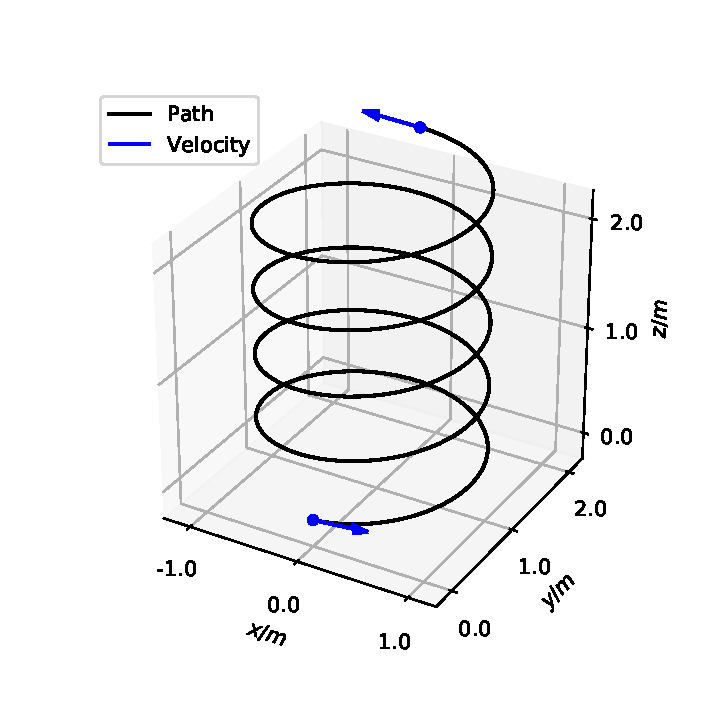
\includegraphics[width=0.4\textwidth]{uniform.pdf}
    \caption{The path of an electron moving in a uniform magnetic field. The field strength is \SI{3.05e-5}{\tesla} in the $z$-direction, and the particle is released at the origin with initial velocity $\begin{bmatrix}\SI{500}{\kilo \meter /\second} & \SI{0}{\kilo \meter /\second} & \SI{50}{\kilo \meter /\second}\end{bmatrix}$}
    \label{fig:uniform}
\end{figure}

The Earth's magnetic field can be modelled as an ideal magnetic dipole. By using the magnitude of the field at the magnetic equator, which is approximately $\SI{3e-5}{T}$~\cite{Lang2010}, one can calculate that a dipole moment of $\SI{8e22}{\ampere \meter^2}$ placed at the center of the Earth will generate a field of this strength at the surface. The orientation of the Earth's field is such that the magnetic south pole points towards the northern hemisphere.

The Earth's axial inclination is approximately \ang{23} \cite{nasa2014}, and the geomagnetic poles (the poles that most closely fit the model where the field of a single bar magnet generates the Earth's magnetic field) are tilted approximately \ang{9} from the geographical poles \cite{kyoto2020}. This leads to an angle between the geomagnetic poles and the ecliptic poles that varies between approximately \ang{14} and \ang{32} during the course of single a day.

The field of a magnetic dipole in a vacuum can be expressed in the form
\begin{equation}
\bm{B} = \frac{\mu_0}{4\pi r^3} \big[3(\bm{m}\cdot\bm{\hat{r}})\bm{\hat{r}} - \bm{m} \big],
\label{eq:mag_dipole}
\end{equation}
where $\mu_0$ is the magnetic permeability of free space, $r$ is the distance from the origin, $\bm{\hat{r}}$ is the unit vector pointing away from the origin, and $\bm{m}$ is the magnetic dipole moment placed at the origin \cite[p.~255]{Griffiths2017}. By switching to Cartesian coordinates and letting the magnetic dipole moment point along the $z$-axis, the field can be written as
\begin{equation}
    \bm{B} = \frac{\mu_0 m (\bm{\hat{x}}\cdot3xz + \bm{\hat{y}}\cdot3yz + \bm{\hat{z}}\cdot(2z^2 -x^2 - y^2))}{4 \pi (x^2 + y^2 + z^2)^{5/2}},
\end{equation}
where $m = \left|\bm{m}\right|$, and $\bm{\hat{x}}$, $\bm{\hat{y}}$ and $\bm{\hat{z}}$ are the unit vectors in the $x$-, $y$-, and $z$-directions respectively. The field is shown in figure \ref{fig:field}.

\begin{figure}[h]
    \centering
    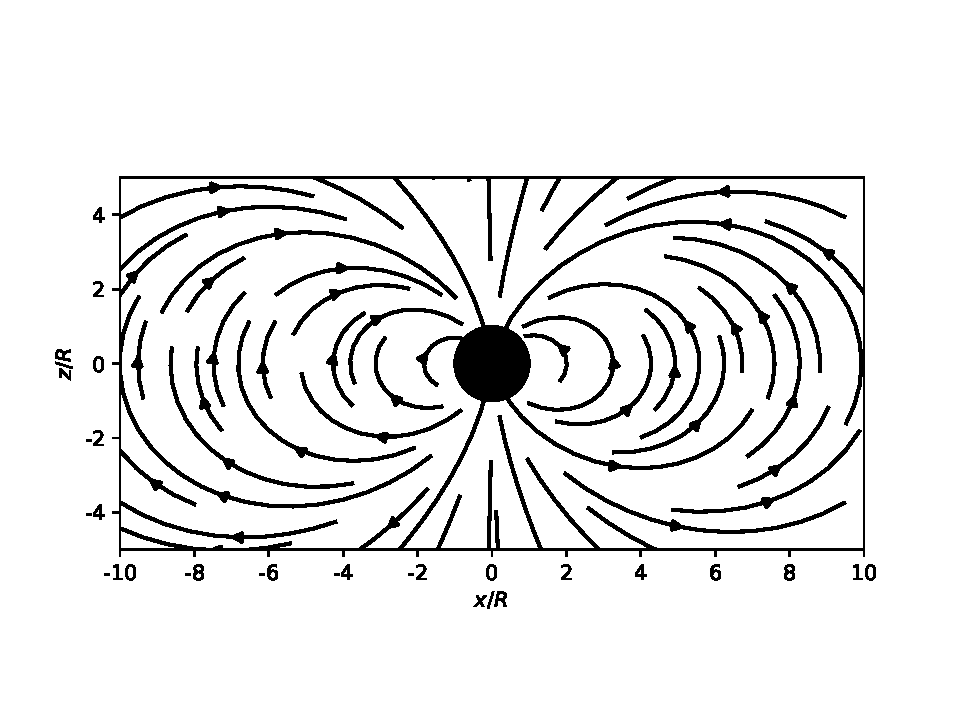
\includegraphics[width=0.45\textwidth]{field.pdf}
    \caption{The Earth's magnetic field approximated as an ideal magnetic dipole. $R$ is the radius of the Earth.}
    \label{fig:field}
\end{figure}

\section{Method}
The Runge-Kutta fourth-order method is used to solve the equation of motion for a particle moving in a general magnetic field. Timesteps are chosen by inspecting the trajectories in the general area where the particle is to move around and ensuring that the motion is sufficiently smooth and does not change when the timestep is decreased. To confirm that the numerical error is negligible, the speed of the particle is compared with its initial speed to ensure that it has not changed.

Particles with an initial speed of \SI{500}{\kilo \meter /\second} are sent towards the earth and their trajectories are inspected. Since their greater mass causes the radius of curvature to be greater, alpha particles are used. This allows a greater timestep to be used in the Runge Kutta method.

For simplicity, the magnetic moment of the Earth is chosen to point in the negative $z$-direction. The angle between the geomagnetic poles and the velocity vector of an incoming particle from the Sun can be anywhere between $\pm \ang{34}$ depending on the time of day and the time of year, thus the chosen angle between them is completely arbitrary and might as well be zero to simplify the calculations.

\section{Results}
Particles were found to spiral around the magnetic field, with their path corresponding to a helix with an axis in the same general direction as the field lines. The pitch of the helix (the distance between two points after completing a full revolution) decreases as the magnetic field increases in size, as seen in figure \ref{fig:helical1}.

\begin{figure}[h]
    \centering
    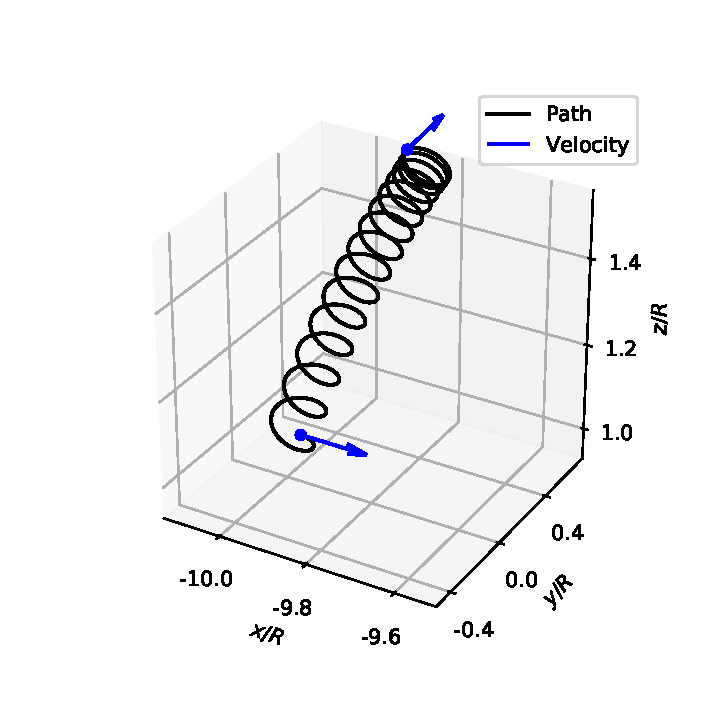
\includegraphics[width=0.4\textwidth]{figure1.pdf}
    \caption{The path of an alpha particle in the Earth's magnetic field. The particle is released at $\begin{bmatrix} -10R&0R&R \end{bmatrix}$ with initial velocity $\begin{bmatrix} \SI{500}{\kilo \meter /\second}&\SI{0}{\kilo \meter /\second}&\SI{0}{\kilo \meter /\second} \end{bmatrix}$. $R$ is the radius of the Earth.}
    \label{fig:helical1}
\end{figure}

Changing the direction of the particle's initial velocity was found to influence the radius and pitch of the helix. It did not, however, affect the overall trajectory of the particle. This is demonstrated in figure \ref{fig:helical2}, where a velocity with direction closer to the field lines causes a smaller radius and a larger pitch.

\begin{figure}[h]
    \centering
    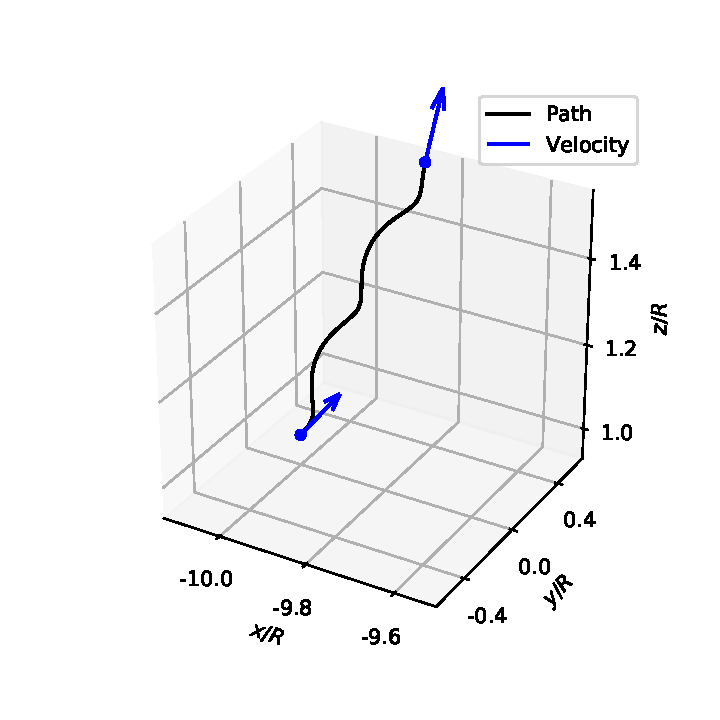
\includegraphics[width=0.4\textwidth]{figure0.pdf}
    \caption{The path of an alpha particle in the Earth's magnetic field. The particle is released at $\begin{bmatrix} -10R&0R&R \end{bmatrix}$ with initial velocity $\begin{bmatrix} \SI{300}{\kilo \meter /\second}&\SI{0}{\kilo \meter /\second}&\SI{400}{\kilo \meter /\second} \end{bmatrix}$. $R$ is the radius of the Earth.}
    \label{fig:helical2}
\end{figure}

As the pitch approaches zero, the helical motion eventually starts moving in approximately the opposite direction. This is demonstrated in figure \ref{fig:helical3}. Notice that the trajectory shifts westward along the azimuth.

\begin{figure}[h]
    \centering
    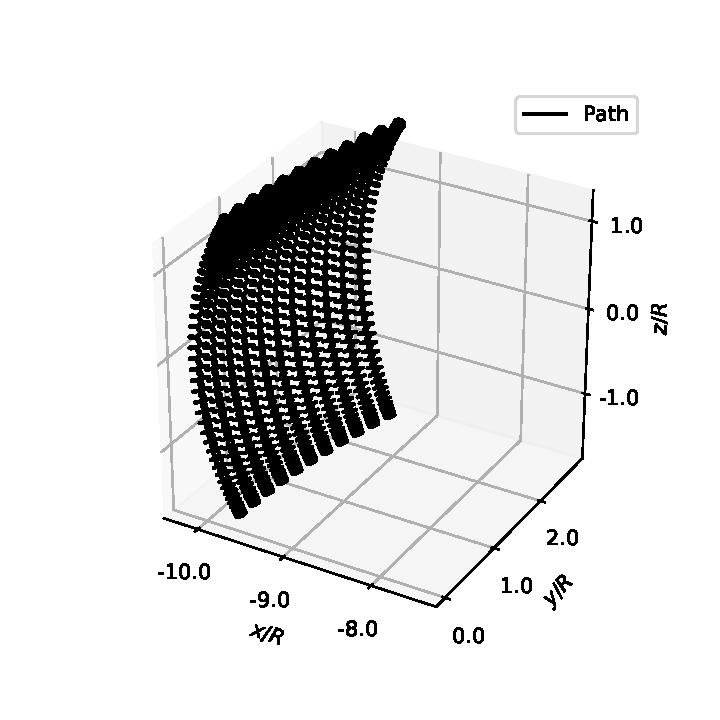
\includegraphics[width=0.4\textwidth]{figure2.pdf}
    \caption{The path of an alpha particle in the Earth's magnetic field. The particle is released at $\begin{bmatrix} -10R&0R&R \end{bmatrix}$ with initial velocity $\begin{bmatrix} \SI{500}{\kilo \meter /\second}&\SI{0}{\kilo \meter /\second}&\SI{0}{\kilo \meter /\second} \end{bmatrix}$. $R$ is the radius of the Earth.}
    \label{fig:helical3}
\end{figure}

\section{Discussion}
Since it is their general behavior in close proximity to the Earth that is of interest, how the particles initially enter and become trapped in the Earth's magnetic field is considered outside the scope of this discussion.

The trajectories deviate from those in a uniform magnetic field with a change of radius, pitch and axis of the helical motion. The axis closely follows the curved field lines, but since the field is stronger at positions closer to the Earth, the radius of curvature is not constant during a full revolution. As a positively charged particle moves clockwise in the magnetic field, which is pointing up, the changing radius of curvature causes it to be deflected westwards.

With the axis of the helix not being in the exact same direction as the field lines, the component of the particle's velocity that points in the direction of the axis changes, allowing the helical motion to eventually slow down and turn around. The particle thus experiences a spiralling motion that oscillates up and down and eventually orbits the earth along the azimuth, as seen in figure \ref{fig:helical3}.

Spiralling trajectories that allow the particles to enter the Earth's atmosphere before the motion turns around could help explain how the aurorae arise. If there are some specific latitudes (with respect to the magnetic poles) that contain trajectories that particles are inclined to enter, it explains why the phenomenon only occurs in locations with some characteristic distance from the Earth's magnetic poles. To fully explain how particles ejected from the Sun could enter such trajectories it would be necessary to consider the actual magnetic field of the Earth, and not just a simplified dipole model.

\section{Conclusion}
As expected from considering the classical example of a charged particle moving in a uniform electric field, the movement of charged particles in the Earth's magnetic field approximated as a magnetic dipole is helical. Since the field strength is greater closer to the Earth, the radius of curvature is not constant during a single revolution. Although the axis of the helical motion curves with the field lines, the changing curvature causes it to not perfectly coincide with a single line as it does in the uniform case, and the trajectory shifts along the azimuth. This motion in turn allows the velocity component along the axis to change since it is not parallel to the field lines. This leads to the oscillatory motion in figure \ref{fig:helical3}.

\begingroup
\begin{center}
\rule{2cm}{.4pt}
\end{center}
\makeatletter
\@beginparpenalty=10000
\makeatother
\bibliographystyle{babunsrt}
\bibliography{references}
\endgroup

\end{document}